\documentclass[10pt,conference,a4paper]{IEEEtran}

\usepackage[T1]{fontenc}
\usepackage{amsmath,amssymb}
\usepackage{graphicx}
\usepackage{booktabs}
\usepackage{multirow}
\usepackage{array}
\usepackage{xcolor}
\usepackage[hidelinks]{hyperref}
\usepackage{cite}
\usepackage{tikz}
\usepackage{algorithm}
\usepackage{algpseudocode}
\usetikzlibrary{arrows.meta,positioning}

\graphicspath{{figures/}}
\newcommand{\sig}[1]{\textbf{#1}}
\setcounter{tocdepth}{2}

\begin{document}
\pagestyle{plain}

\definecolor{covernavy}{HTML}{1F3A5F}
\definecolor{coveraccent}{HTML}{A8432F}
\definecolor{covergrey}{HTML}{5A6878}
\begin{titlepage}
\raggedright
\vspace*{0.5cm}
{\color{covernavy}\rule{\textwidth}{2.5pt}}\par
\vspace{2mm}
\IfFileExists{figures/usyd_logo.png}{\includegraphics[height=1.6cm]{usyd_logo.png}}{{\small\bfseries\color{covernavy}THE UNIVERSITY OF SYDNEY}}\hfill{\small\color{covergrey}ELEC5305 \textperiodcentered{} Semester 2, 2026}\par
\vspace{5.5cm}
{\small\bfseries\color{coveraccent}FINAL PROJECT REPORT\par}
\vspace{4mm}
{\fontsize{26}{31}\selectfont\bfseries\color{covernavy}How Quickly Should a Speech\\[1mm] Enhancer Adapt?\par}
\vspace{5mm}
{\Large\color{covergrey}Change-Aware Wiener Filtering under Abrupt Background-Noise Changes\par}
\vfill
{\color{covernavy}\rule{\textwidth}{0.6pt}}\par
\vspace{3mm}
\renewcommand{\arraystretch}{1.35}
\begin{tabular}{@{}>{\color{covergrey}}l@{\hspace{8mm}}l@{}}
Author & \textbf{Liya Xu} \\
SID & 530519058 \\
Unit of study & ELEC5305 Acoustics, Speech and Signal Processing \\
Submitted & 13 November 2026 \\
Code and results & \url{https://github.com/Liyaxuxu/elec5305-project-530519058} \\
Project website & \url{https://liyaxuxu.github.io/elec5305-project-530519058/} \\
Video demonstration & \url{https://youtu.be/natY-4UzcTU} \\
Video (backup copy) & \url{https://drive.google.com/file/d/1G7SuL2PIYqyZcJeBJBOGOTtxOiQHFxEb/view} \\
\end{tabular}\par
\vspace{3mm}
{\color{covernavy}\rule{\textwidth}{2.5pt}}\par
\end{titlepage}

\begin{titlepage}
\small
\renewcommand{\contentsname}{\large Contents}
\tableofcontents
\vfill
\end{titlepage}


\begin{abstract}
A causal STFT speech enhancer has to re-estimate the noise every time the
background changes, and for a short time after the change it can either leave
the new noise in or damage the speech. This project asks one question: how
quickly should such an enhancer adapt after an abrupt change, and does a
lightweight change-aware controller help compared with fixed and SNR-only
control? I kept one Wiener enhancement equation and only changed the
controller: fixed, SNR-only, two change-aware controllers, an always-fast
controller and an oracle that knows the true change time. All systems were
tested on controlled VoiceBank/DEMAND mixtures with level, type, onset and
offset changes. Settings were chosen on one speaker and frozen before testing
on a validation split and on an office-to-cafeteria split never used during
development. The improvement followed the time spent in the fast state: across
the eight Wiener controllers this fraction correlated with SI-SDR at $r=0.97$
(validation) and $r=0.95$ (unseen test), and the
always-fast controller beat both change-aware controllers on both splits, so
change detection did not add value on these scenes. All classical systems
failed at the moment of change: none removed a newly started noise within
0.75~s, all kept suppressing speech after the noise stopped, and none improved
STOI. A pretrained DeepFilterNet3 reference improved SI-SDR by about 9--11~dB
over the best Wiener controller and was the only system that improved STOI.
\end{abstract}

\begin{IEEEkeywords}
speech enhancement, Wiener filter, noise tracking, non-stationary noise, change
detection, transient evaluation
\end{IEEEkeywords}

\section{Introduction}

Most speech enhancement examples assume that the background noise is
stationary. In practice it is not: an air conditioner switches on, a person
walks from an office into a cafeteria, or traffic gets louder. Speech
enhancement is now used in devices that run continuously, such as hearing aids,
conferencing systems and phones, so the noise environment can change many times
after the system is deployed. Recent work has started to study this problem for
neural enhancers, for example lightweight adaptation over sequences of changing
acoustic scenes~\cite{cheng2026lightweight}, while other work focuses on keeping
latency low enough for interactive use~\cite{wu2025ultralow,kim2026laco}.

Classical enhancers face the same problem in a very visible way. A Wiener
filter is only as good as its noise estimate, and that estimate is a recursive
average with a time constant. If the time constant is long, the estimate cannot
follow a new noise; if it is short, speech leaks into the noise estimate and is
suppressed. The noise-tracking literature has mostly attacked this trade-off by
designing better estimators~\cite{martin2001noise,gerkmann2012unbiased}, and
enhancers are usually evaluated with averages over whole utterances. What has
received less attention is what happens in the short interval right after a
change, and whether simply \emph{switching} the adaptation speed at the right
time is a cheap alternative to a better estimator.

This project therefore addresses a single research question:
\begin{quote}
\emph{When the acoustic environment changes abruptly, how quickly should a
causal STFT speech enhancer adapt, and can a lightweight change-aware controller
reduce adaptation delay and speech distortion compared with fixed and SNR-only
baselines?}
\end{quote}
Two sub-questions help to answer it: (a) do normal whole-utterance metrics hide
short failures right after the change, and (b) how does this interpretable
system compare with a pretrained real-time neural enhancer?

I kept the scope narrow. I do not train a neural model or propose a
new noise estimator. I take a standard Wiener filter, keep its gain rule fixed
and change only the controller that sets the noise and gain smoothing. An
oracle controller that knows the true change time separates detector errors from
controller errors, and an always-fast controller tests whether detecting the
change is needed at all.

The contributions are: (i) a controlled dynamic-scene protocol with known
change times, measured SNRs and no-change controls; (ii) a transition-centred
evaluation with settling time and a speech/noise error decomposition; (iii) a
controller ablation with paired statistics on a validation split and an unseen
transition pair; and (iv) a ``Dynamic
Speech Enhancement Auditor'' tool that produces all diagnostics for one scene.
Section~\ref{sec:lit} reviews the literature, Section~\ref{sec:method}
describes the method, Section~\ref{sec:results} presents the results and
Section~\ref{sec:discussion} discusses them.

\section{Literature Review}
\label{sec:lit}

I grouped the literature into five themes: classical enhancement, noise
tracking, temporal change cues, neural streaming enhancement and evaluation
practice. For each I summarise what is known and what it means for my question.

\subsection{Classical enhancement and the role of the noise estimate}
Spectral subtraction~\cite{boll1979spectral} subtracts an estimate of the noise
magnitude spectrum from the noisy spectrum. Berouti et
al.~\cite{berouti1979enhancement} added an over-subtraction factor and a
spectral floor to reduce musical noise. The Wiener filter applies a gain
$G=\xi/(1+\xi)$, where $\xi$ is the a~priori SNR, and Scalart and
Filho~\cite{scalart1996apriori} showed that a smoothed (decision-directed)
estimate of $\xi$ gives a more stable gain. All of these methods share one
weak point: they assume the noise estimate is correct. When the noise changes,
the gain is computed from an out-of-date estimate, so noise-estimation error is
an important source of error right after a change, although the gain floor, the
gain smoothing and the SNR estimate also affect it. I used the same gain rule in
every system so that the comparison is controlled, and varied only how fast the
noise estimate and the gain are allowed to move.

\subsection{Noise tracking: delay versus speech leakage}
The literature offers three main ways to track noise, and they make different
compromises (Table~\ref{tab:tracking}). A \emph{recursive average} updated
mostly when speech is absent is simple, but its speed is fixed by its smoothing
coefficient. Martin's \emph{minimum statistics}~\cite{martin2001noise} tracks
the minimum of a smoothed power spectrum over about 1.5~s; it works during
speech because speech rarely fills every frame of a bin, but a rising noise can
only be followed after the old minimum leaves the window. Gerkmann and
Hendriks~\cite{gerkmann2012unbiased} use the speech presence probability in an
MMSE estimator, which reduces tracking delay to a few hundred milliseconds while
keeping speech leakage low. The common theme is a trade-off between tracking
delay and speech leakage, which the methods handle with different assumptions
and update rules. My
project tests a different idea: keep the simple recursive tracker, but move
along the trade-off over time, fast only when the scene seems to change.

\begin{table}[t]
\centering
\caption{Noise-tracking approaches and their behaviour at a scene change.}
\label{tab:tracking}
\footnotesize
\begin{tabular}{@{}p{2.0cm}p{2.7cm}p{2.8cm}@{}}
\toprule
Method & Strength & Weakness at a change\\
\midrule
Recursive average (VAD- or SNR-weighted) & Simple, interpretable, one parameter & Fixed speed; a big noise rise can look like speech and is not tracked\\
Minimum statistics~\cite{martin2001noise} & Works during speech & Rise only tracked after $\approx$1.5~s window\\
MMSE / SPP~\cite{gerkmann2012unbiased} & Low delay, low speech leakage & More complex; still a fixed compromise\\
\textbf{This project}: recursive + controller & Speed can change over time & Depends on detecting the change\\
\bottomrule
\end{tabular}
\end{table}

\subsection{Temporal and modulation cues for change detection}
Speech and environmental noise have different temporal patterns. Paliwal et
al.~\cite{paliwal2009modulation} applied spectral subtraction in the modulation
domain and showed that information across frames helps to separate them. I did
not reproduce their algorithm; it motivated using simple temporal change cues
(log-spectral change, spectral flux and short-time subband modulation) as scene
detectors. The obvious risk, which the proposal feedback also pointed out, is
that speech itself changes quickly, so a large spectral change does not always
mean the noise changed. This is why detection was evaluated separately, with
no-change controls.

\subsection{Neural and streaming enhancement}
Neural enhancers now run in real time. DeepFilterNet~\cite{schroter2023deepfilternet}
is an open, pretrained full-band model. Wu and Braun~\cite{wu2025ultralow}
studied ultra-low-latency enhancement and note that hearing applications may need
latencies below about 5~ms, and LaCo-SENet~\cite{kim2026laco} treats latency as
a configurable trade-off against quality. Cheng and
Liu~\cite{cheng2026lightweight} studied post-deployment adaptation of neural
enhancers over sequences of 111 environments and 37 noise types. Compared with
classical trackers, these models learn the noise statistics implicitly and can
react within a few frames, but they are harder to inspect and much heavier to
train. They are the current state of the art for quality; they do not make the
classical question irrelevant, because a cheap, interpretable controller is still
attractive for low-power devices.

\subsection{Evaluation practice}
Enhancement is usually evaluated with utterance-level quality and intelligibility
measures. Loizou and Kim~\cite{loizou2011reasons} showed that improving quality
measures often does not improve intelligibility, mainly because over-suppression
removes speech cues, so I report STOI~\cite{taal2011stoi} next to the
distortion measure SI-SDR~\cite{leroux2019sdr}. For my question, an utterance average can hide a short failure: 500~ms of poor
enhancement after a change barely moves a 6--8~s average but can contain a whole
word. The classical papers I read~\cite{boll1979spectral,scalart1996apriori,loizou2011reasons}
report results as averages over whole utterances, and the tracking papers mainly
report how fast the noise estimate follows a change rather than what happens to
the enhanced speech in that interval~\cite{martin2001noise,gerkmann2012unbiased}.
Measuring the enhanced speech right after the change is the evaluation gap this
project tries to fill.

\subsection{Available code and choice of approach}
Table~\ref{tab:approaches} lists the code I considered. MATLAB's Signal
Processing Toolbox provides \texttt{stft}/\texttt{istft} and the Audio
Toolbox provides \texttt{stoi}; the VOICEBOX toolbox~\cite{brookes_voicebox}
implements \texttt{specsub} with minimum-statistics and MMSE trackers; and the
DeepFilterNet repository provides pretrained models and a Python interface. The
Wiener filter, controllers, detectors and evaluation were written for this
project instead of being taken from a toolbox, so that every internal quantity
could be logged; VOICEBOX and DeepFilterNet3 are used only as references. Training a neural model was out of scope.

\begin{table}[t]
\centering
\caption{Code and approaches considered, and their role here.}
\label{tab:approaches}
\footnotesize
\begin{tabular}{@{}p{2.2cm}p{2.7cm}p{2.6cm}@{}}
\toprule
Approach / code & Advantage & Disadvantage / role\\
\midrule
Own spectral subtraction~\cite{boll1979spectral} & Simple, cheap & Fixed noise. Baseline.\\
Own Wiener + recursive tracker~\cite{scalart1996apriori} & Interpretable state, causal & Tracker speed is a trade-off. \textbf{Main system.}\\
VOICEBOX \texttt{specsub}~\cite{brookes_voicebox} & Published trackers~\cite{martin2001noise,gerkmann2012unbiased} & GPL; not modified. Reference.\\
DeepFilterNet3~\cite{schroter2023deepfilternet} & Best quality, real time & Black box, heavier. Reference only.\\
Model adaptation~\cite{cheng2026lightweight} & Adapts to new scenes & Needs training. Not used.\\
\bottomrule
\end{tabular}
\end{table}

\subsection{Concepts I had to learn}
Several ideas were new to me. \emph{SI-SDR}~\cite{leroux2019sdr} measures
distortion after optimal scaling of the reference, so it does not depend on the
output level. \emph{STOI}~\cite{taal2011stoi} predicts intelligibility from the
correlation of short-time temporal envelopes. \emph{Causality} means a decision
at time $t$ may only use samples up to $t$; I checked it with tests that change
the future part of a signal and confirm that past gains do not change. The
\emph{time constant} of a recursive average with coefficient $\alpha$ and hop
$T$ is roughly $T/(1-\alpha)$, which turned out to be the key to interpreting
the results. Finally, the \emph{cluster bootstrap}~\cite{efron1993bootstrap}
resamples whole speech sequences, because the eight cases built from one
sequence are not independent, and a \emph{difference-in-differences} test
compares an improvement in one condition with the same improvement in another.

\subsection{Research gap}
So the literature offers better trackers, better neural models and many
utterance-level evaluations, but I did not find a controlled study that keeps the
enhancer fixed, varies only the adaptation speed over time, and evaluates the
interval right after the change with an oracle and no-change controls. That is
the gap this project addresses, at a course-project scale.

\section{Method}
\label{sec:method}

\subsection{How the method answers the question}
The research question is about \emph{adaptation speed} and \emph{change
detection}. Each part of the design isolates one factor
(Table~\ref{tab:design}). If the change-aware controller beats fixed and
SNR-only control, adapting at the change helps. If the oracle is much better
than the detector-driven controller, the detector is the bottleneck. If the
always-fast controller is as good or better, the timing information is not
needed and speed alone explains the gain. The transition metrics answer
sub-question (a), and the reference systems answer sub-question (b).

\begin{table}[t]
\centering
\caption{Design elements and what each one tests.}
\label{tab:design}
\footnotesize
\begin{tabular}{@{}p{2.8cm}p{4.9cm}@{}}
\toprule
Design element & What it isolates\\
\midrule
Same STFT, gain rule, tracker & Differences come only from the controller.\\
Fixed vs SNR-only vs change & Benefit of adapting at the change.\\
Oracle trigger & Detector error vs controller error.\\
Always fast & Whether timing (detection) is needed at all.\\
Level / type / onset / offset & Which kinds of change benefit (feedback hypothesis).\\
Speech-active vs pause & Speech interference with the detector.\\
No-change controls & False alarms, cost of adapting when nothing changed.\\
Development-only tuning & Prevents fitting to the test data.\\
Unseen transition pair & Generalisation beyond the tuning noises.\\
Transition metrics & Short failures hidden by averages (sub-question a).\\
VOICEBOX, DeepFilterNet3 & Context against published methods (sub-question b).\\
\bottomrule
\end{tabular}
\end{table}

\subsection{Overview}
Fig.~\ref{fig:pipeline} shows the pipeline. A clean utterance is mixed with
noise~A before a known change time and noise~B after it. Every Wiener system
processes the same mixture with the same STFT and gain rule; only the
controller differs. The outputs are scored over the whole signal and in the
interval right after the change.

\begin{figure}[t]
\centering
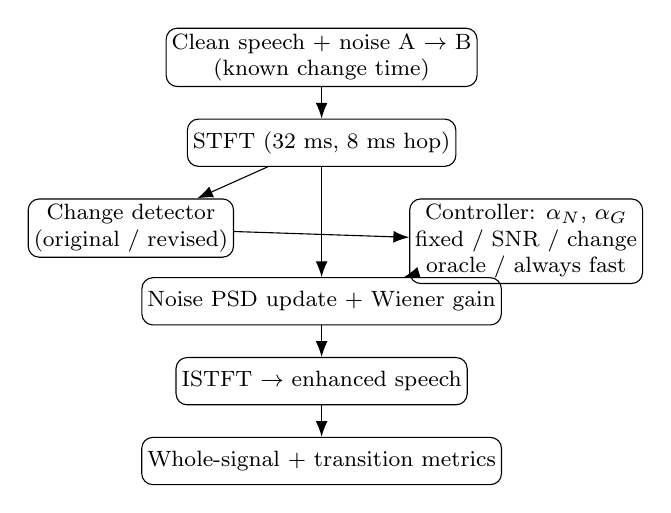
\begin{tikzpicture}[node distance=4mm, every node/.style={font=\footnotesize},
box/.style={draw, rounded corners, align=center, minimum height=6mm, inner sep=2pt},
arr/.style={-{Latex[length=2mm]}}]
\node[box] (mix) {Clean speech + noise A $\to$ B\\(known change time)};
\node[box, below=of mix] (stft) {STFT (32 ms, 8 ms hop)};
\node[box, below left=4mm and -6mm of stft] (det) {Change detector\\(original / revised)};
\node[box, below right=4mm and -6mm of stft] (ctl) {Controller: $\alpha_N$, $\alpha_G$\\fixed / SNR / change\\oracle / always fast};
\node[box, below=14mm of stft] (gain) {Noise PSD update + Wiener gain};
\node[box, below=of gain] (istft) {ISTFT $\to$ enhanced speech};
\node[box, below=of istft] (met) {Whole-signal + transition metrics};
\draw[arr] (mix) -- (stft);
\draw[arr] (stft) -- (det);
\draw[arr] (det) -- (ctl);
\draw[arr] (ctl) -- (gain);
\draw[arr] (stft) -- (gain);
\draw[arr] (gain) -- (istft);
\draw[arr] (istft) -- (met);
\end{tikzpicture}
\caption{Experimental pipeline. All Wiener systems share the STFT, noise update
and gain rule; only the controller changes.}
\label{fig:pipeline}
\end{figure}

\subsection{Wiener enhancer}
The noisy signal is analysed with a 512-sample (32~ms) periodic Hamming window
and a 128-sample (8~ms) hop at 16~kHz. For frame $m$ and bin $k$, with noisy
power $P(k,m)=|Y(k,m)|^2$ and noise estimate $\hat\lambda(k,m)$, I use the
instantaneous a~priori SNR
\begin{equation}
\xi(k,m)=\max\!\left(\frac{P(k,m)}{\hat\lambda(k,m-1)}-1,\;0\right),
\end{equation}
which is simpler than the decision-directed estimate of~\cite{scalart1996apriori}.
The noise estimate is updated with a step that shrinks when the bin is likely
to contain speech, and the observation is capped to avoid jumps:
\begin{align}
\mu(k,m)&=\frac{1-\alpha_N(m)}{1+\xi(k,m)},\\
\hat\lambda(k,m)&=(1-\mu)\,\hat\lambda(k,m-1)+\mu\min\!\big(P,\,6\hat\lambda(k,m-1)\big).
\end{align}
The target gain is $G_t=\max(\xi/(1+\xi),G_{\min})$ with $G_{\min}=0.05$, and it
is smoothed over time:
\begin{equation}
G(k,m)=\alpha_G(m)\,G(k,m-1)+(1-\alpha_G(m))\,G_t(k,m).
\end{equation}
With an 8~ms hop, the slow noise coefficient $\alpha_N=0.995$ corresponds to a
time constant of about 1.6~s and the fast value $\alpha_N=0.90$ to about 80~ms
(before the speech weighting in (2), which slows the update further). Each case
starts with 0.5~s of noise only; during this calibration prefix the noise
estimate is the running mean of past frames only.

The experiments are offline simulations, not a streaming implementation: for
convenience the STFT of the whole recording is computed in one call. What is
causal is the frame-level processing. The noise estimate, the controller
decision and the gain for frame $m$ use only frames up to $m$, and a frame counts
as available 16~ms after its centre, when all of its samples have arrived. The
automated tests check this by changing the later part of a signal and confirming
that earlier gains and detector decisions do not change.

\subsection{Controllers}
The controllers only set $\alpha_N$ and $\alpha_G$ (Table~\ref{tab:controllers}).
Smaller values mean faster adaptation. The change-aware controllers switch to a
``fast state'' for a hold time after each detector trigger. I also tested a
linear release ramp back to the slow state and a larger gain floor.

\begin{table}[t]
\centering
\caption{Controllers. Slow state: $\alpha_N=0.995$, $\alpha_G=0.90$. Fast state
(selected on development data): $\alpha_N=0.90$, $\alpha_G=0.75$.}
\label{tab:controllers}
\footnotesize
\begin{tabular}{@{}p{2.1cm}p{5.6cm}@{}}
\toprule
Controller & Rule\\
\midrule
Fixed & Always slow.\\
SNR-only & $\alpha_N=0.995-0.055w$, $\alpha_G=0.90-0.20w$, $w=\mathrm{clip}\big((5-\mathrm{SNR_{dB}})/15,0,1\big)$.\\
Change (orig./rev.) & Fast for 0.35~s after each trigger of the original or revised detector.\\
SNR + change & SNR rule, but the faster of the two rates is used during the fast state.\\
Always fast & Fast state in every frame.\\
Oracle & Fast for 0.35~s from the true change time (diagnostic only).\\
\bottomrule
\end{tabular}
\end{table}

\subsection{Change detectors}
The \emph{original} detector computes three causal scores: the mean distance
between the current log spectrum and a smoothed log spectrum, positive spectral
flux of the normalised magnitude spectrum, and the change in short-time
modulation energy of eight subband log energies. Each score is normalised by the
median and median absolute deviation of its previous 1~s, the maximum of the
three is compared with 6, and two consecutive frames above threshold trigger a
0.35~s hold.

The \emph{revised} detector was designed to reduce false alarms caused by speech.
It tracks the 20th percentile of eight subband energies, compares the last
0.20~s with the 0.65~s before it, and uses the median absolute band change in dB
as the score. The threshold is $8+0.75\max(E-6,0)$~dB, where $E$ is how far the
current energy is above the floor (a rough sign of speech), and four consecutive
frames are required. These settings were chosen on development data from a grid
of 48 combinations and frozen.

\subsection{Dynamic scenes and data splits}
Clean speech comes from the VoiceBank test set~\cite{valentini2017voicebank} and
noise from DEMAND~\cite{thiemann2013demand}. Each case is 8~s long: a 0.5~s
noise-only prefix followed by 7.5~s of speech, made by joining eight consecutive
utterances and cutting the result to length. The change point is
chosen at random from an active-speech region between 2.5 and 4.5~s, so most
changes happen while the person is talking. Each speech sequence gives five
change cases and three no-change controls:
\begin{itemize}
\item \emph{level}: noise~A rises by 10~dB;
\item \emph{type}: noise~A $\to$ noise~B at similar power;
\item \emph{onset}/\emph{offset}: noise~B starts from, or drops to, a $-30$~dB floor;
\item \emph{type\_pause}: same as type, but the speech is faded to silence for 0.5~s around the change;
\item controls: stationary noise~A, stationary noise~B, clean speech only.
\end{itemize}
In an earlier version the ``quiet'' side of onset and offset was digital
silence. With an all-zero prefix every noise tracker I tried, including VOICEBOX,
stayed at zero, so onsets could not be measured; the $-30$~dB floor fixes this.
The real SNR before and after each change is saved in the manifests.

Table~\ref{tab:splits} lists the splits. Six sequences per split give 48 cases.
The two-speaker VoiceBank test subset I used contains only p232 and p257, and
both are used (one for development, one for testing), so \textbf{the final test
uses unseen utterances, noise excerpts and an unseen transition pair, but not an
unseen speaker}.

\begin{table}[t]
\centering
\caption{Data splits (6 speech sequences, 48 cases each).}
\label{tab:splits}
\footnotesize
\begin{tabular}{@{}lllp{2.4cm}@{}}
\toprule
Split & Speaker & Noise A$\to$B & Use\\
\midrule
Development & p232 & office$\to$traffic & choose detector and controller settings\\
Validation & p257 & office$\to$traffic & frozen test (looked at once before)\\
Unseen test & p257 & office$\to$\textbf{cafeteria} & final test, new utterances and pair\\
\bottomrule
\end{tabular}
\end{table}

\subsection{Reference systems}
Three references do not depend on the controller: (i) fixed magnitude spectral
subtraction (over-subtraction 1.5, floor 0.03, noise from the first 250~ms);
(ii) VOICEBOX \texttt{specsub} in Wiener mode with the MMSE noise
tracker~\cite{gerkmann2012unbiased,brookes_voicebox}; and (iii) pretrained
DeepFilterNet3~\cite{schroter2023deepfilternet}, run in Python at 48~kHz with
16$\to$48$\to$16~kHz resampling. VOICEBOX is GPL licensed, so it is used locally
and not redistributed in the repository.

\subsection{Metrics}
Over the whole signal I report SI-SDR~\cite{leroux2019sdr}, segmental SNR (32~ms
frames with speech, clamped to $[-10,35]$~dB~\cite{loizou2013speech}), its
improvement over the noisy input, STOI~\cite{taal2011stoi} and runtime. Around
the change I report SI-SDR in the first 0.75~s (\emph{transition SI-SDR}),
SI-SDR 1.5--2.5~s later (\emph{steady state}), and the \emph{settling time}: the
start of the first three consecutive 100~ms blocks whose error energy is within
1.5~dB of the median error measured from 1.5~s after the change. Some cases never
settle within the recording. Mean settling times are computed only over the
cases that settled (between 14 and 20 of the 24 level, type, onset and offset
cases, depending on the system and split), and paired comparisons keep only the
cases where both systems settled. Because each
Wiener system saves its gain matrix, I also apply that gain separately to the
clean speech and to the added noise, which gives the transition speech
distortion and residual-noise suppression. Detectors are scored by hit rate
within 1.5~s, delay and false alarms per minute, including on no-change
controls.

The clean-speech control is excluded from all averages, because the Wiener
systems reproduce it exactly and its SI-SDR is undefined. The type\_pause case is
excluded from transition averages because the reference is silent right at the
change.

\subsection{Parameter selection and statistics}
The fast-state settings (fast $\alpha_G\in\{0.55,0.75\}$, hold
$\in\{0.35,0.70\}$~s, release $\in\{0,0.30\}$~s, $G_{\min}\in\{0.05,0.10\}$)
were chosen on the development split only, using the oracle trigger so that
detector errors could not affect the choice. The objective was mean whole-signal
plus mean transition SI-SDR. The selected setting (fast $\alpha_G=0.75$, hold
0.35~s, no release, $G_{\min}=0.05$) was then frozen; the full search is in
Appendix~\ref{app:search}. Note that this search objective was averaged over
all development cases, so its transition term includes the type\_pause case,
while the final tables use the narrower sets described above. All comparisons
are paired by case, and 95\%
intervals come from a cluster bootstrap over the six sequences with 5000
resamples. I call a difference significant when its interval excludes zero; with
six sequences this is a small sample.

\subsection{Full intended method and what was not completed}
The full method I planned also included a test speaker never seen before, and
combining the change trigger with a stronger (MMSE) noise tracker. I did not
keep an unseen speaker because both speakers of the test subset were already
used; other VoiceBank speakers could be added later. Combining the trigger with an MMSE
tracker is left as future work (Section~\ref{sec:future}).

\subsection{Implementation and new tools}
Everything except DeepFilterNet3 is written in MATLAB (Signal Processing and
Audio Toolboxes). New to me were MATLAB's \texttt{stft}/\texttt{istft}
reconstruction conventions (a Hann window with zero end points caused large
errors at the signal edges in my spectral subtraction, which I fixed with a
periodic Hamming window), running a pretrained PyTorch model from Python, and
writing automated tests for causality and gain decomposition. All results are
produced by scripts in the repository (Appendix~\ref{app:repro}). The main files
are \texttt{src/transition\_wiener.m} (enhancer and controllers),
\texttt{src/scene\_change\_detector.m} and
\texttt{src/robust\_change\_features.m} (detectors),
\texttt{src/run\_controller\_ablation.m} (experiment) and
\texttt{src/summarise\_controller\_ablation.m} (statistics); the core loop is
listed in Appendix~\ref{app:code}.

\section{Results}
\label{sec:results}

\subsection{Sanity check of the Wiener filter}
Before the dynamic experiments I checked the fixed Wiener filter on the
stationary development cases (Table~\ref{tab:refcheck}). Its SI-SDR is in the
same range as the same gain rule with the \emph{true} noise PSD and as the
VOICEBOX references, so the basic implementation behaves as expected.

\begin{table}[t]
\centering
\caption{Stationary-noise check: mean SI-SDR (dB), 6 cases each.}
\label{tab:refcheck}
\footnotesize
\begin{tabular}{@{}lrr@{}}
\toprule
System & Office & Traffic\\
\midrule
Noisy input & 0.37 & 0.40\\
My fixed Wiener & 6.39 & 4.24\\
Same gain, true noise PSD & 5.99 & 4.90\\
VOICEBOX min.\ statistics & 2.60 & 3.55\\
VOICEBOX MMSE & 4.56 & 5.40\\
\bottomrule
\end{tabular}
\end{table}

\subsection{Detector audit}
Table~\ref{tab:detector} compares the two detectors on the validation split
(this audit used the earlier digital-silence onsets; per-condition results are
in Appendix~\ref{app:detector}). The revised detector found more changes, much
faster, with fewer false alarms on no-change controls, but its false alarms on
clean speech rose from 65.7 to 98.6 per minute: without a steady noise floor the
low percentile follows the gaps between syllables. Of the false alarms, 67.2\%
(original) and 44.2\% (revised) fell within 100~ms of a speech onset, which
supports the feedback's concern that speech onsets are mistaken for scene
changes. Even though the revised detector was the better detector, the enhancer
using it scored lower SI-SDR. The next sections explain why.

\begin{table}[t]
\centering
\caption{Detector audit on the validation split (48 cases).}
\label{tab:detector}
\footnotesize
\begin{tabular}{@{}lrr@{}}
\toprule
& Original & Revised\\
\midrule
Changes detected within 1.5 s & 20/30 & 23/30\\
False alarms/min, no-change controls & 62.4 & 41.9\\
Mean delay of detected changes (s) & 0.62 & 0.18\\
Enhancer SI-SDR (dB) & 4.51 & 3.61\\
\bottomrule
\end{tabular}
\end{table}

\subsection{Main comparison}
Table~\ref{tab:main} gives the main results. All Wiener controllers improve
SI-SDR over the noisy input, and the overall trend is similar on both splits:
fixed and SNR-only are lowest, the oracle and the controllers using the revised
detector come next, the controllers using the original detector are higher, and
always-fast is the best Wiener controller on both splits. The exact order is not
identical (fixed and SNR-only swap places, for example). Spectral subtraction and VOICEBOX are better than all my Wiener
controllers, and DeepFilterNet3 is far ahead of everything. No classical system
improves STOI; DeepFilterNet3 is the only one above the noisy input.

\begin{table*}[t]
\centering
\caption{Main results (42 cases with noise, frozen setting). $\Delta$SSNR:
segmental-SNR improvement over noisy. FF: fraction of time in the fast state
(validation/unseen).}
\label{tab:main}
\small
\setlength{\tabcolsep}{6pt}
\begin{tabular}{@{}lrrrrrrr@{}}
\toprule
& \multicolumn{3}{c}{Validation} & \multicolumn{3}{c}{Unseen test} & \\
\cmidrule(lr){2-4}\cmidrule(lr){5-7}
System & SI-SDR & $\Delta$SSNR & STOI & SI-SDR & $\Delta$SSNR & STOI & FF\\
\midrule
Noisy & 1.17 & 0.00 & .806 & 1.10 & 0.00 & .767 & --\\
Fixed & 3.22 & 1.17 & .800 & 2.97 & 0.85 & .756 & 0\\
SNR-only & 3.32 & 1.33 & .800 & 2.87 & 0.85 & .757 & 0\\
Oracle & 3.56 & 1.65 & .801 & 3.24 & 1.17 & .757 & .03\\
Change (rev.) & 3.66 & 1.87 & .801 & 3.31 & 1.36 & .755 & .15/.17\\
SNR+chg.\ (rev.) & 3.71 & 1.79 & .799 & 3.27 & 1.23 & .755 & .15/.17\\
Change (orig.) & 4.38 & 2.11 & .803 & 3.57 & 1.30 & .755 & .35/.38\\
SNR+chg.\ (orig.) & 4.39 & 2.11 & .800 & 3.55 & 1.33 & .754 & .35/.38\\
Always fast & 5.33 & 2.77 & .804 & 4.04 & 1.78 & .754 & 1\\
\midrule
Spectral sub. & 7.20 & 3.80 & .806 & 5.76 & 3.13 & .760 & --\\
VOICEBOX MMSE & 6.02 & 3.46 & .804 & 4.20 & 2.16 & .756 & --\\
DeepFilterNet3 & \sig{16.05} & \sig{8.90} & \sig{.837} & \sig{13.50} & \sig{7.98} & \sig{.804} & --\\
\bottomrule
\end{tabular}
\end{table*}

Table~\ref{tab:paired} shows the key paired differences. The pattern becomes
clear when the controllers are ordered by the fraction of time they spend in the
fast state (last column of Table~\ref{tab:main}): the oracle is fast only 3\% of
the time, the revised detector about 16\%, the original detector 35--38\%
(because of its many false alarms) and always-fast 100\%. Across the eight
Wiener controllers this fraction correlates with whole-signal SI-SDR at $r=0.97$
(validation) and $r=0.95$ (unseen test). This explains the surprising result that
the original change-aware controller beats the oracle by 0.82~dB and 0.32~dB even
though the oracle knows the true change time.

\begin{table*}[t]
\centering
\caption{Paired differences A$-$B with 95\% cluster-bootstrap intervals. Bold:
interval excludes zero. Trans.: transition SI-SDR over level, type, onset, offset.}
\label{tab:paired}
\small
\setlength{\tabcolsep}{8pt}
\begin{tabular}{@{}lll@{}}
\toprule
A $-$ B (metric) & Validation & Unseen test\\
\midrule
Always fast $-$ fixed (SI-SDR) & \sig{+2.11} [1.74, 2.48] & \sig{+1.07} [0.78, 1.33]\\
Change orig.\ $-$ fixed (SI-SDR) & \sig{+1.16} [0.95, 1.35] & \sig{+0.60} [0.26, 0.95]\\
SNR-only $-$ fixed (SI-SDR) & +0.10 [$-$0.09, 0.27] & $-$0.10 [$-$0.22, 0.01]\\
Always fast $-$ change orig. (SI-SDR) & \sig{+0.95} [0.57, 1.35] & \sig{+0.47} [0.26, 0.66]\\
Change orig.\ $-$ oracle (SI-SDR) & \sig{+0.82} [0.59, 1.02] & \sig{+0.32} [0.03, 0.63]\\
Oracle $-$ fixed (trans.) & \sig{+0.84} [0.54, 1.24] & \sig{+0.58} [0.02, 1.01]\\
Oracle $-$ change orig.\ (trans.) & +0.03 [$-$0.27, 0.33] & $-$0.39 [$-$0.68, 0.03]\\
Oracle $-$ always fast (trans.) & \sig{$-$0.59} [$-$0.92, $-$0.25] & $-$0.49 [$-$1.02, 0.11]\\
Fixed $-$ noisy (STOI) & \sig{$-$0.005} [$-$0.009, $-$0.001] & \sig{$-$0.011} [$-$0.014, $-$0.008]\\
DFN3 $-$ noisy (STOI) & \sig{+0.032} [0.023, 0.039] & \sig{+0.037} [0.027, 0.049]\\
\bottomrule
\end{tabular}
\end{table*}

Most of the always-fast advantage is not at the change itself. In the steady
state 1.5--2.5~s after a level change, always-fast reaches 4.22~dB SI-SDR on
validation against 1.66~dB for fixed, a much larger gap than in the transition
interval (2.11 vs 1.39~dB); the same holds for type changes (4.57 vs 1.48~dB in
the steady state). The no-change controls show the same thing for two of the three noises: with
nothing changing, always-fast gained 2.3~dB over fixed on stationary traffic and
0.6~dB on stationary cafeteria noise, but nothing on office noise ($+0.1$~dB on
validation, $-0.3$~dB on the unseen test). Steady-state values for the other
conditions are in Appendix~\ref{app:condition}.

Fig.~\ref{fig:modern} compares the controllers with the reference systems. The
classical systems all run at a real-time factor of about 0.006 on my CPU (about
0.045~s for an 8~s signal), while DeepFilterNet3 needs about 0.36~s (real-time
factor about 0.05), so it is roughly eight times slower but still well within
real time.

\begin{figure*}[t]
\centering
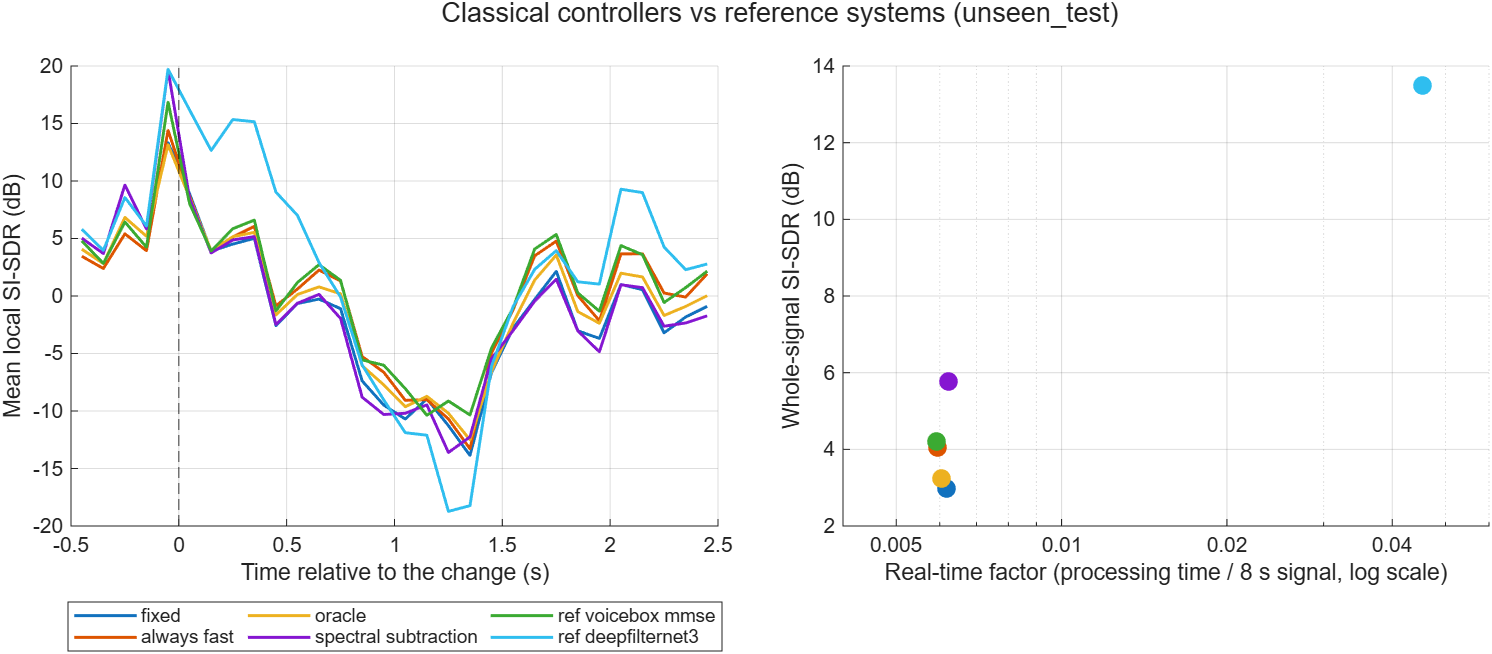
\includegraphics[width=0.74\textwidth]{modern_reference_unseen.png}
\caption{Unseen test. Left: mean local SI-SDR in 100~ms blocks around the change
(level, type, onset, offset). Right: whole-signal SI-SDR against real-time
factor. DeepFilterNet3 is far ahead on quality at roughly eight times the
runtime of the classical systems.}
\label{fig:modern}
\end{figure*}

\subsection{Behaviour at each type of change}
Table~\ref{tab:condition} shows the transition SI-SDR for each type of change.
Two failures stand out.

\textbf{Onset.} When noise starts, no classical system improves on the noisy
input by more than 0.8~dB in the first 0.75~s, including VOICEBOX, and the
residual-noise suppression in this interval is below 1~dB for every Wiener
controller. For my tracker the reason is visible in Fig.~\ref{fig:onset}: after a
sudden 30~dB rise the a~priori SNR $\xi$ becomes very large, so the update step
$\mu$ in (2) is almost zero and the capped observation in (3) is still close to
the old estimate. The fixed tracker treats the new noise as speech and hardly
updates at all; the always-fast tracker does climb, but it needs about one second
to approach the new level, which is longer than the 0.75~s transition window.
DeepFilterNet3 reaches about 9--10~dB immediately.

\textbf{Offset.} After the noise stops, the input is almost clean (about 30~dB
SI-SDR), but every classical system drops to 11--18~dB because the old, high
noise estimate keeps suppressing speech. Here fast adaptation helps: the original
change-aware controller is 2.5~dB (validation) and 2.4~dB (unseen) better than
SNR-only, and both differences are significant.

For level and type changes, the oracle and always-fast controllers are the best
Wiener systems, but they gain at most about 1~dB over the fixed controller.

\begin{table*}[t]
\centering
\caption{Transition SI-SDR (dB, first 0.75~s) by type of change.}
\label{tab:condition}
\small
\setlength{\tabcolsep}{7pt}
\begin{tabular}{@{}lrrrrrrrr@{}}
\toprule
& Noisy & Fixed & SNR-only & Change (orig.) & Always fast & Oracle & VOICEBOX & DFN3\\
\midrule
\multicolumn{9}{@{}l}{\emph{Validation}}\\
Level & $-$0.86 & 1.39 & 1.27 & 1.31 & 2.11 & 2.20 & 1.02 & 15.56\\
Type & $-$0.60 & 2.71 & 2.61 & 2.91 & 3.48 & 3.53 & 2.96 & 12.85\\
Onset & $-$0.60 & $-$0.59 & $-$0.48 & $-$0.18 & 0.18 & $-$0.55 & $-$0.29 & 10.48\\
Offset & 29.34 & 11.04 & 11.28 & 13.75 & 14.50 & 12.74 & 18.27 & 16.67\\
\midrule
\multicolumn{9}{@{}l}{\emph{Unseen test}}\\
Level & 0.32 & 2.55 & 2.31 & 2.21 & 3.04 & 3.19 & 1.95 & 18.97\\
Type & 0.16 & 2.58 & 2.47 & 2.70 & 2.73 & 2.75 & 2.46 & 9.97\\
Onset & 0.16 & 0.15 & 0.23 & 0.44 & 0.67 & 0.22 & 0.35 & 9.44\\
Offset & 30.18 & 10.90 & 12.32 & 14.69 & 14.00 & 12.31 & 18.06 & 17.43\\
\bottomrule
\end{tabular}
\end{table*}

\begin{figure}[t]
\centering
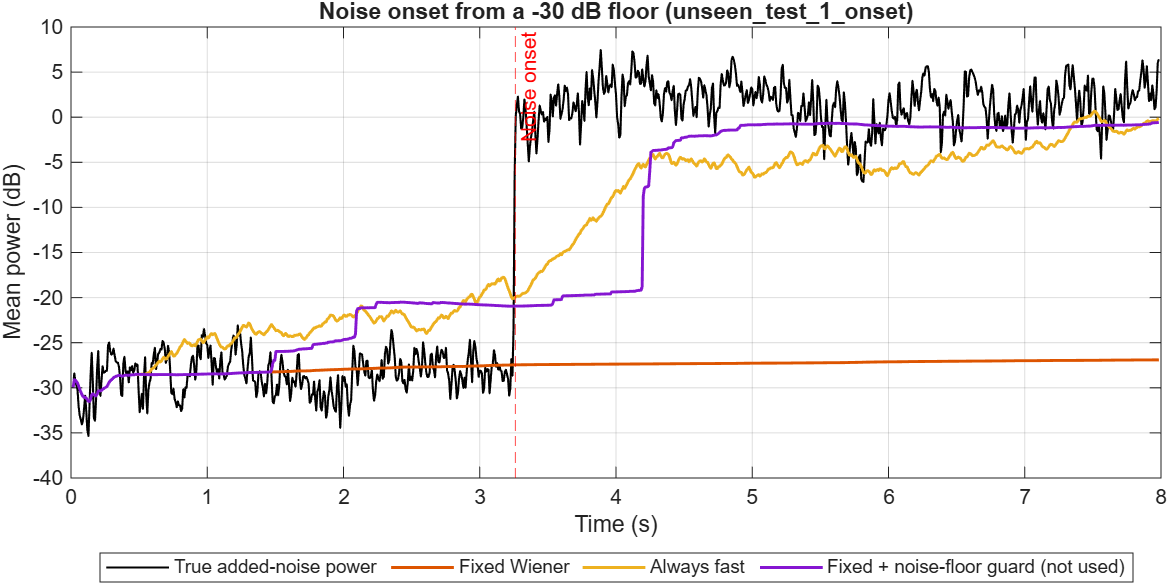
\includegraphics[width=\columnwidth]{onset_noise_estimate_unseen.png}
\caption{Mean noise estimate around a noise onset (first unseen-test onset
case). After the 30~dB rise the fixed tracker stays at the old floor and the
always-fast tracker needs about one second to approach the new level. An
experimental noise-floor guard jumps up faster but overestimated noise during
speech, so it was not used.}
\label{fig:onset}
\end{figure}

Fig.~\ref{fig:settling} shows the settling time per condition. It should be read
together with the error level: settling time only says when the error becomes
stable, not how good it is, and the fixed controller never settles after an
offset within the recording on the unseen test (missing bar). The oracle settles
fastest after level changes; the SNR+change controller with the revised cue
settles slowly in several conditions, which matches its repeated triggers.

\begin{figure}[t]
\centering
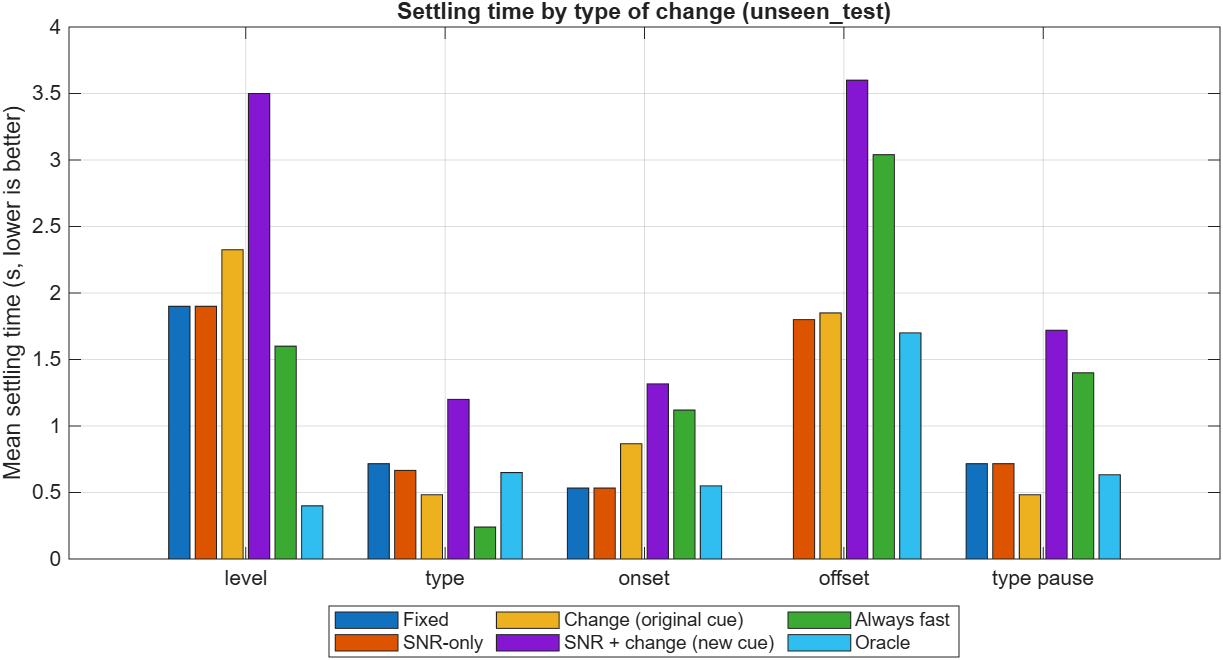
\includegraphics[width=\columnwidth]{settling_unseen.png}
\caption{Mean settling time by type of change (unseen test).}
\label{fig:settling}
\end{figure}

Fig.~\ref{fig:tradeoff} shows the trade-off between speech distortion and
residual noise in the transition interval. The faster controllers reach lower
speech error but suppress less of the new noise, and the fixed controller is at
the other end. No controller is better on both axes, which is the trade-off
described in the noise-tracking literature.

\begin{figure}[t]
\centering
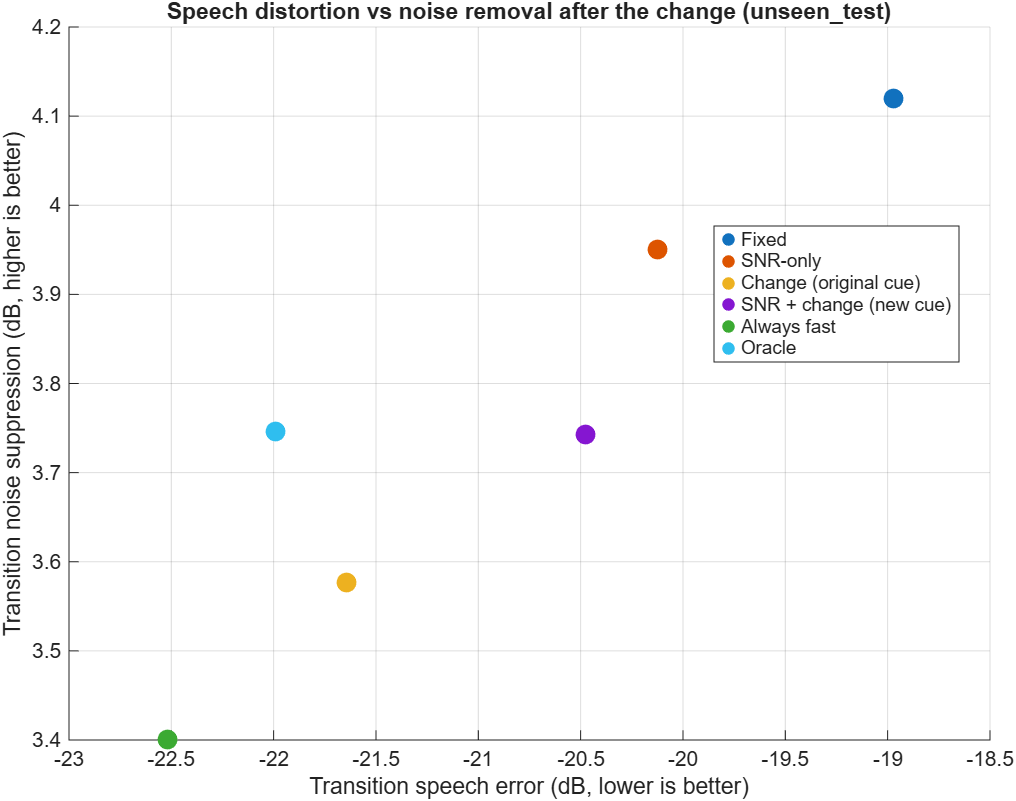
\includegraphics[width=0.9\columnwidth]{tradeoff_unseen.png}
\caption{Transition speech error against transition noise suppression (unseen
test). Left is less speech damage, up is more noise removed.}
\label{fig:tradeoff}
\end{figure}

\subsection{Testing the hypothesis from the proposal feedback}
The hypothesis was that SNR-only adaptation handles level changes, while a
spectral/modulation change cue helps more when the noise \emph{type} changes at a
similar level. I tested it directly as a difference-in-differences: (change $-$
SNR-only) for type changes minus the same difference for level changes. On
validation the original cue gave $+0.26$~dB [$-0.21$, $0.70$], not significant.
On the unseen test the revised cue was significantly \emph{worse} for type changes
than for level changes ($-0.49$~dB [$-1.05$, $-0.11$]). So the hypothesis was not
supported. The condition where the change cue clearly helped was the offset
(previous subsection).

\subsection{Do averages hide transition failures?}
Fig.~\ref{fig:avgtrans} plots whole-signal metrics against transition SI-SDR.
Ranking the systems by whole-signal SI-SDR and by transition SI-SDR gives a rank
correlation of 0.91 (validation) and 0.81 (unseen), so the overall ranking
mostly agrees. However, the averages hide the condition-specific failures in
Table~\ref{tab:condition}: the onset is almost not enhanced at all, and the
offset damages clean speech. The oracle is also a good example: it ranks low on
the whole signal but is among the best right after level and type changes.

\begin{figure}[t]
\centering
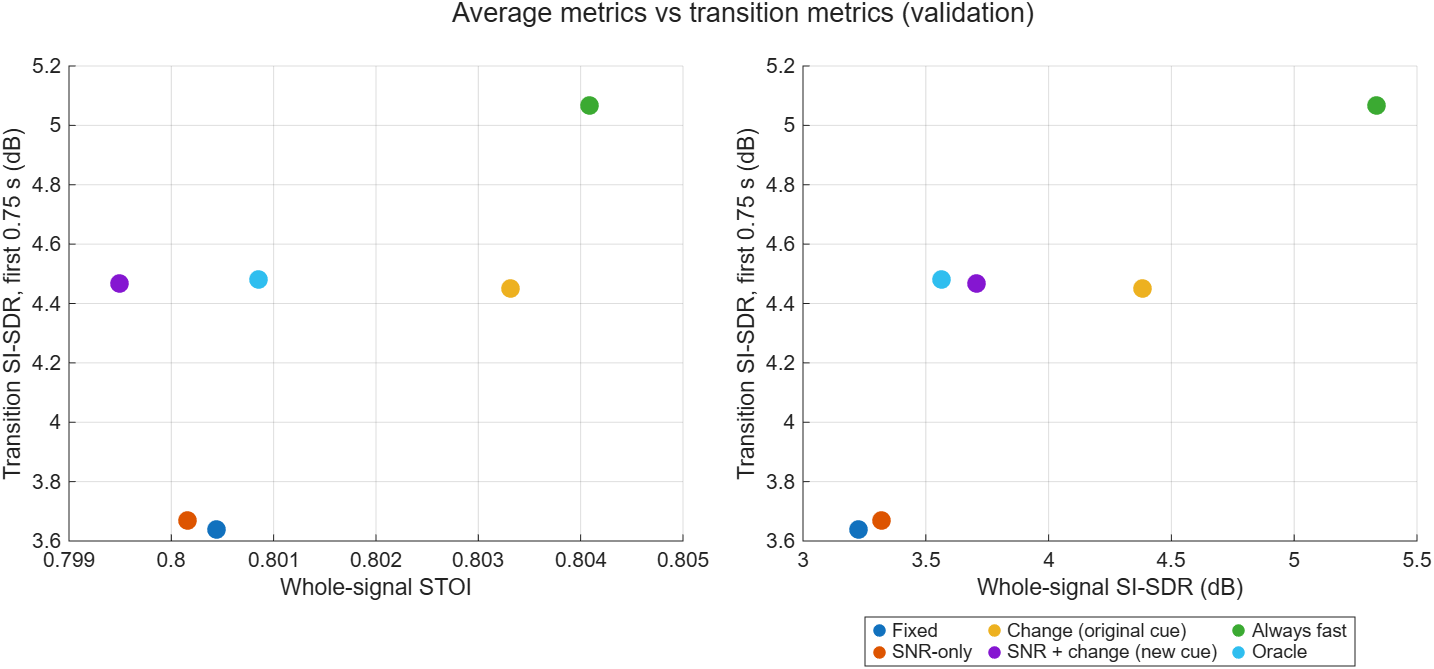
\includegraphics[width=\columnwidth]{average_vs_transition_validation.png}
\caption{Whole-signal STOI (left) and SI-SDR (right) against transition SI-SDR
(validation).}
\label{fig:avgtrans}
\end{figure}

\subsection{Auditor example}
Fig.~\ref{fig:auditor} shows the Dynamic Speech Enhancement Auditor on one
office-to-cafeteria change at 5~dB SNR, with unused p257 speech. The example was
chosen by a fixed rule (the first excerpt in a fixed scan where the revised
detector finds the change); here the first excerpt already qualified, with a
delay of 80~ms and one false alarm. It is an illustration of the tool, not a
typical case, and it does not follow the same start-up protocol as the main
experiments: this 6~s example has no noise-only prefix and initialises the noise
estimate from the first 250~ms of the mixture.
The noise estimates of the slow controllers barely move after the change, while
the faster controllers lower their gain within about half a second.

\begin{figure*}[t]
\centering
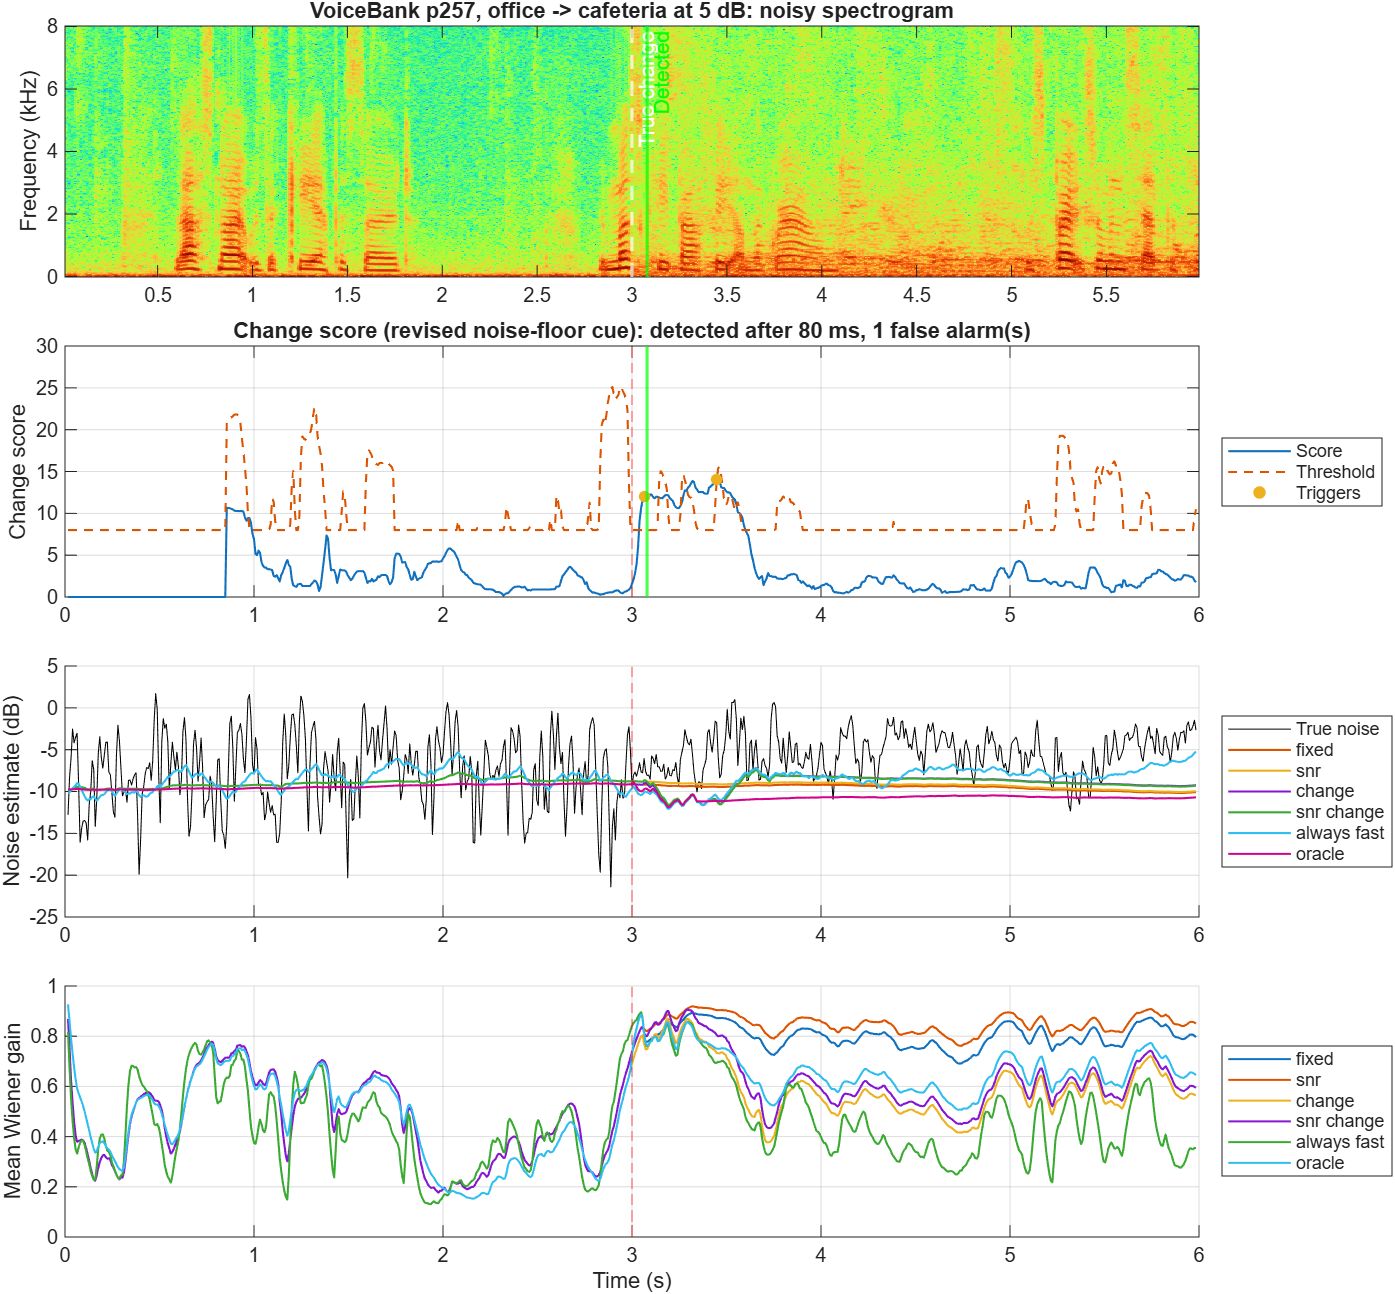
\includegraphics[width=0.68\textwidth]{auditor_overview.png}
\caption{Auditor output for one office-to-cafeteria change (selected example).
From top: noisy spectrogram with true (white) and detected (green) change;
revised change score, threshold and triggers; mean noise estimate of each
controller against the true noise power; mean Wiener gain.}
\label{fig:auditor}
\end{figure*}

\subsection{Sources of error}
Several things limit how precise these numbers are. The intervals come from only
six speech sequences, so each difference has to be judged by its own bootstrap
interval, and the small sample limits how far the results generalise. SI-SDR
is undefined when an output reproduces the reference exactly, so those cases are
dropped, which is why the clean control is excluded everywhere. Local SI-SDR in
100~ms blocks is noisy when the speech in the block is quiet, so the recovery
curve in Fig.~\ref{fig:modern} should be read qualitatively, and settling time
can be misleading when the error never reaches a stable level. DeepFilterNet3
runs at 48~kHz, so its input and output are resampled, which may cost it a small
amount of SI-SDR. Finally, the validation split had already been used once in
the detector audit, so the cafeteria split is the only completely fresh test.

\section{Discussion}
\label{sec:discussion}

\subsection{Answering the research question}
A change-aware controller did reduce distortion compared with the fixed and
SNR-only baselines: the original change-aware controller improved SI-SDR by
1.16~dB (validation) and 0.60~dB (unseen) over fixed, and it helped most after
the noise stopped. But the always-fast controller, which uses no detection, was
better on both splits, and the oracle, which has perfect timing, scored below
the detector with the most false alarms. On these scenes my answer to ``how
quickly should the enhancer adapt?'' is therefore: faster than my slow setting,
and not only at the detected changes. This answers the question only partly. It
holds for these office, traffic and cafeteria recordings and for this simple
tracker.

The time constants offer one possible explanation. The slow setting averages the
noise over about 1.6~s and the fast setting over about 80~ms (longer in
practice because of the speech weighting). If the noise level moves on a shorter
time scale than 1.6~s, the fixed controller works with an out-of-date estimate
even when the scene does not change, and a detector that fires only at scene
changes cannot repair that. The no-change controls fit this picture if traffic and
cafeteria noise fluctuate more than office noise: the fast setting helped on the
first two and not on the third. But I did not measure how fast the noise level
fluctuates and I did not sweep the slow coefficients, so this explanation is not
tested directly.

For sub-question (a), whole-signal numbers gave a similar overall ranking but
hid the two most important failures, at onsets and offsets, which only appear
when the change interval is evaluated separately for each type of change. For
sub-question (b), DeepFilterNet3 was much better on whole-signal SI-SDR,
segmental SNR and STOI, and it handled onsets immediately, at about eight times
the runtime of the classical systems. It was not best on every measure: on the
unseen test its mean settling time (1.66~s) was longer than the oracle's
(0.62~s), and VOICEBOX had a higher transition SI-SDR after offsets. The value of
the classical system is that its failures can be traced to its internal state,
as in Fig.~\ref{fig:onset}.

\subsection{Comparison with the literature}
The lack of STOI improvement for all classical systems agrees with Loizou and
Kim~\cite{loizou2011reasons}: lower distortion did not translate into better
predicted intelligibility. The onset failure is the textbook weakness of a
speech-weighted recursive tracker: a sudden rise in noise looks exactly like
speech onset. Minimum statistics and MMSE trackers~\cite{martin2001noise,gerkmann2012unbiased}
were designed to reduce this, and indeed VOICEBOX MMSE was better than my
controllers overall. It still did not remove onsets within 0.75~s, which is
consistent with its tracking delay being short but not zero. The large gap to
DeepFilterNet3 matches the direction of the field towards learned streaming
enhancers~\cite{schroter2023deepfilternet}, and the importance of fast
adaptation after a change agrees with the motivation of~\cite{cheng2026lightweight}.

\subsection{Alternative explanations}
The slow setting may simply have been a poor choice. The slow coefficients were
kept from the earlier experiments and the development search only changed the
fast state, so a better-tuned fixed controller might close part of the gap to
always-fast. Whether a detector helps on top of a better-tuned baseline remains
untested.

The choice of metric also matters. SI-SDR rewards strong suppression, which is
probably why spectral subtraction scores well. This is the reason STOI and the
speech/noise decomposition are reported next to it; in that decomposition the
faster controllers had lower speech error, not higher
(Fig.~\ref{fig:tradeoff}).

The oracle should not be read as an upper bound. It removes detector errors but
keeps the same fast-state setting, so it shows whether timing helps, not the
best result that could be achieved. Finally, six sequences per split is a small
sample. The main statements above rest on differences whose intervals excluded
zero on both the validation and the unseen split; smaller effects are reported
as uncertain.

\subsection{What worked and what did not}
The protocol worked well: known change times, measured SNRs, no-change controls,
an oracle, development-only tuning and paired statistics made the results easy to
interpret, and the conclusions held on a noise pair never used during
development. Two things did not work. First, the revised detector reduced false
alarms but not distortion. Second, an experimental ``noise-floor guard'' (raising the estimate to
a scaled running minimum) did follow onsets, but it overestimated the noise
during speech and reduced SI-SDR on stationary noise (6.39 to 5.60~dB for
office), so I left it out. It was also surprising that plain spectral
subtraction beat all Wiener controllers. Its noise estimate is fixed, but its
over-subtraction removes more noise, which SI-SDR rewards at these SNRs. This
suggests that my gain rule and tracker are too conservative.

\subsection{Limitations}
(i) No unseen speaker: all tests use p257. (ii) Only six sequences per split and
three DEMAND environments, so the intervals are wide and the results may not
generalise. (iii) The validation split had been looked at once before.
(iv) The detector audit used digital-silence onsets, unlike the final ablation.
(v) The Auditor example was selected to show a detected change. (vi) The slow
setting was not tuned, and I did not measure how fast the noise level
fluctuates. (vii) The experiments are offline simulations with frame-level
causality, not a real-time implementation. Several of these can be addressed:
more VoiceBank training speakers and DEMAND environments would solve
(i)--(iii), and including the slow coefficients in the development search would
address (vi).

\subsection{Future work}
\label{sec:future}
The most promising next step is to replace my speech-weighted tracker with an
MMSE or minimum-statistics tracker and then test whether a change trigger still
adds anything on top of it, since such trackers already handle continuous
fluctuations. A faster release after offsets, more speakers and more noise
environments would also make the conclusions stronger. A small listening test focused on the first second after each change
would also show whether the measured differences are audible.

\section{Conclusion}
I built a controlled experiment to measure how quickly a Wiener speech enhancer
with frame-level causal processing should adapt after an abrupt noise change.
With one shared enhancement equation and only the controller changed, an
always-fast controller beat both change-aware controllers on a validation split
and on an unseen office-to-cafeteria split, so accurate change detection did not
translate into better enhancement here. A likely reason is that the slow setting
could not follow the ordinary fluctuations of the traffic and cafeteria noise,
but this was not tested directly. Evaluating the interval right after the change
showed two failures that whole-signal averages hide: a newly started noise is
not removed within 0.75~s, and speech is over-suppressed after the noise stops.
A pretrained neural reference did much better on the whole-signal metrics at a
modest runtime cost. The code, results and the Auditor tool are available in the
project repository.

\section*{Use of AI tools}
AI was primarily used to improve the grammar, clarity, and fluency of the writing in this report. It was also used to refine the readability and coherence of the code. All final content was reviewed and verified by the author.

\bibliographystyle{IEEEtran}
\bibliography{references}

\clearpage
\appendices

\section{Development search for the controller setting}
\label{app:search}
Table~\ref{tab:search} lists all 16 fast-state settings evaluated on the
development split with the oracle trigger. The objective is mean whole-signal
SI-SDR plus mean transition SI-SDR. The fast noise coefficient was fixed at
$\alpha_N=0.90$. The selected row is in bold.

\begin{table}[h]
\centering
\caption{Development controller search (oracle trigger, p232).}
\label{tab:search}
\scriptsize
\begin{tabular}{@{}rrrrrrr@{}}
\toprule
Fast $\alpha_G$ & Hold & Release & $G_{\min}$ & Whole & Trans. & Obj.\\
\midrule
0.55 & 0.35 & 0.00 & 0.05 & 3.88 & 0.74 & 4.62\\
0.55 & 0.35 & 0.00 & 0.10 & 3.83 & 0.62 & 4.45\\
0.55 & 0.35 & 0.30 & 0.05 & 3.89 & $-$0.35 & 3.55\\
0.55 & 0.35 & 0.30 & 0.10 & 3.84 & $-$0.06 & 3.79\\
0.55 & 0.70 & 0.00 & 0.05 & 3.92 & 0.48 & 4.41\\
0.55 & 0.70 & 0.00 & 0.10 & 3.87 & 0.40 & 4.28\\
0.55 & 0.70 & 0.30 & 0.05 & 3.92 & 0.53 & 4.45\\
0.55 & 0.70 & 0.30 & 0.10 & 3.87 & 0.44 & 4.31\\
\textbf{0.75} & \textbf{0.35} & \textbf{0.00} & \textbf{0.05} & \textbf{3.90} & \textbf{0.81} & \textbf{4.70}\\
0.75 & 0.35 & 0.00 & 0.10 & 3.85 & 0.63 & 4.48\\
0.75 & 0.35 & 0.30 & 0.05 & 3.92 & 0.28 & 4.19\\
0.75 & 0.35 & 0.30 & 0.10 & 3.86 & $-$0.25 & 3.62\\
0.75 & 0.70 & 0.00 & 0.05 & 3.95 & 0.56 & 4.51\\
0.75 & 0.70 & 0.00 & 0.10 & 3.90 & 0.24 & 4.14\\
0.75 & 0.70 & 0.30 & 0.05 & 3.95 & 0.57 & 4.53\\
0.75 & 0.70 & 0.30 & 0.10 & 3.90 & 0.25 & 4.15\\
\bottomrule
\end{tabular}
\end{table}

\section{Detector audit by condition}
\label{app:detector}
Table~\ref{tab:detcond} breaks the detector audit down by condition
(validation, digital-silence onsets).

\begin{table}[h]
\centering
\caption{Detector hit rate within 1.5~s and false alarms per minute.}
\label{tab:detcond}
\footnotesize
\begin{tabular}{@{}lrrrr@{}}
\toprule
& \multicolumn{2}{c}{Hit rate} & \multicolumn{2}{c}{False alarms/min}\\
\cmidrule(lr){2-3}\cmidrule(lr){4-5}
Condition & Orig. & Rev. & Orig. & Rev.\\
\midrule
Level & 0.83 & 0.67 & 54.3 & 31.4\\
Type & 0.50 & 0.67 & 47.1 & 11.4\\
Onset & 0.33 & 0.83 & 44.3 & 40.0\\
Offset & 1.00 & 1.00 & 67.1 & 58.6\\
Type during pause & 0.67 & 0.67 & 48.6 & 14.3\\
Stationary office & -- & -- & 65.7 & 27.1\\
Stationary traffic & -- & -- & 55.7 & 0.0\\
Clean speech & -- & -- & 65.7 & 98.6\\
\bottomrule
\end{tabular}
\end{table}

\section{Additional per-condition results}
\label{app:condition}
Tables~\ref{tab:steady} and~\ref{tab:settle} give the steady-state SI-SDR
(1.5--2.5~s after the change) and the settling time.

\begin{table}[h]
\centering
\caption{Steady-state SI-SDR (dB), validation / unseen test.}
\label{tab:steady}
\scriptsize
\setlength{\tabcolsep}{2pt}
\begin{tabular}{@{}lrrrrr@{}}
\toprule
Condition & Fixed & SNR-only & Chg.\ (orig.) & Always fast & Oracle\\
\midrule
Level & 1.66/4.01 & 1.66/3.79 & 3.63/5.17 & 4.22/6.56 & 3.11/5.54\\
Type & 1.48/2.61 & 1.47/2.49 & 2.32/2.64 & 4.57/3.50 & 2.15/2.64\\
Onset & $-$0.75/0.93 & $-$0.69/0.96 & $-$0.35/1.20 & 2.43/2.51 & $-$0.73/0.94\\
Offset & 11.41/11.22 & 16.97/14.60 & 19.45/19.54 & 21.06/21.84 & 13.37/12.50\\
\bottomrule
\end{tabular}
\end{table}

\begin{table}[h]
\centering
\caption{Settling time (s), validation / unseen test. -- = never settled.}
\label{tab:settle}
\scriptsize
\setlength{\tabcolsep}{2pt}
\begin{tabular}{@{}lrrrrr@{}}
\toprule
Condition & Fixed & SNR-only & Chg.\ (orig.) & Always fast & Oracle\\
\midrule
Level & 2.08/1.90 & 1.50/1.90 & 2.97/2.33 & 2.10/1.60 & 3.00/0.40\\
Type & 0.93/0.72 & 0.95/0.67 & 1.00/0.48 & 1.80/0.24 & 2.04/0.65\\
Onset & 1.28/0.53 & 1.28/0.53 & 1.22/0.87 & 1.30/1.12 & 0.98/0.55\\
Offset & 0.15/-- & 3.05/1.80 & 3.00/1.85 & 2.36/3.04 & 2.10/1.70\\
\bottomrule
\end{tabular}
\end{table}

Means cover settled cases only; this metric is a rough diagnostic.

\section{Reproducing the results}
\label{app:repro}
From the repository root in MATLAB, with the datasets placed as described in
\texttt{data/README.md}:

{\footnotesize
\begin{verbatim}
addpath('src');
run('tests/run_tests.m');
run_controller_ablation("develop");
run_controller_ablation("validate");
run_controller_ablation("test");
summarise_controller_ablation;
run('src/run_auditor_example.m');
\end{verbatim}
}

{\raggedright\noindent The stationary reference check
(\texttt{tools/check\_against\_voicebox.m}, Table~\ref{tab:refcheck}) is
optional and needs the VOICEBOX files, which are not included in the repository
because of their GPL licence; they are copied into
\texttt{tools/external/voicebox/} as described in the README. DeepFilterNet3 (optional) is run with
\texttt{python} \texttt{tools/run\_deepfilternet.py} \texttt{data/dfn\_io/<split>} in a Python 3.10
environment from \texttt{tools/requirements-dfn.txt}, after which the ablation
and summary are run again to score it. The controller-ablation tables come from the files in
\texttt{results/controller\_ablation/}: \texttt{*\_final\_table.csv},
\texttt{*\_paired\_bootstrap.csv}, \texttt{*\_by\_condition.csv} and
\texttt{*\_hypothesis\_by\_condition.csv} (DeepFilterNet3 timings:
\texttt{*\_dfn\_runtime.csv}). The detector-audit tables come from
\texttt{results/detector\_revision/} and Table~\ref{tab:refcheck} from
\texttt{results/reference\_check/}.\par}

\section{Core enhancer loop}
\label{app:code}
Algorithm~\ref{alg:loop} summarises the per-frame loop of
\texttt{src/transition\_wiener.m} (full code in the repository).

\begin{algorithm}[H]
\caption{Per-frame Wiener update with controller (simplified)}
\label{alg:loop}
\scriptsize
\begin{algorithmic}[1]
\State $\hat\lambda \gets$ mean of the 0.5~s noise-only prefix
\For{each frame $m$ after the prefix}
  \State $P \gets |Y(\cdot,m)|^2$;\; $\xi \gets \max(P/\hat\lambda-1,0)$
  \State start a 0.35~s hold if the detector fires (change) or $m$ is the true change (oracle)
  \State $(\alpha_N,\alpha_G) \gets (0.90,0.75)$ if always fast or in hold; SNR rule if SNR mode; else $(0.995,0.90)$
  \State $\mu \gets (1-\alpha_N)/(1+\xi)$;\; $\hat\lambda \gets (1-\mu)\hat\lambda+\mu\min(P,6\hat\lambda)$
  \State $G \gets \alpha_G G+(1-\alpha_G)\max(\xi/(1+\xi),0.05)$;\; $\hat S(\cdot,m) \gets G\,Y(\cdot,m)$
\EndFor
\State enhanced signal $\gets$ ISTFT of $\hat S$
\end{algorithmic}
\end{algorithm}

\end{document}
